\documentclass{standalone}
\usepackage{tikz}
\usetikzlibrary{patterns, positioning}
\usepackage[sfdefault]{ClearSans} %% option 'sfdefault' activates Clear Sans as the default text font
\usepackage[T1]{fontenc}

\begin{document}
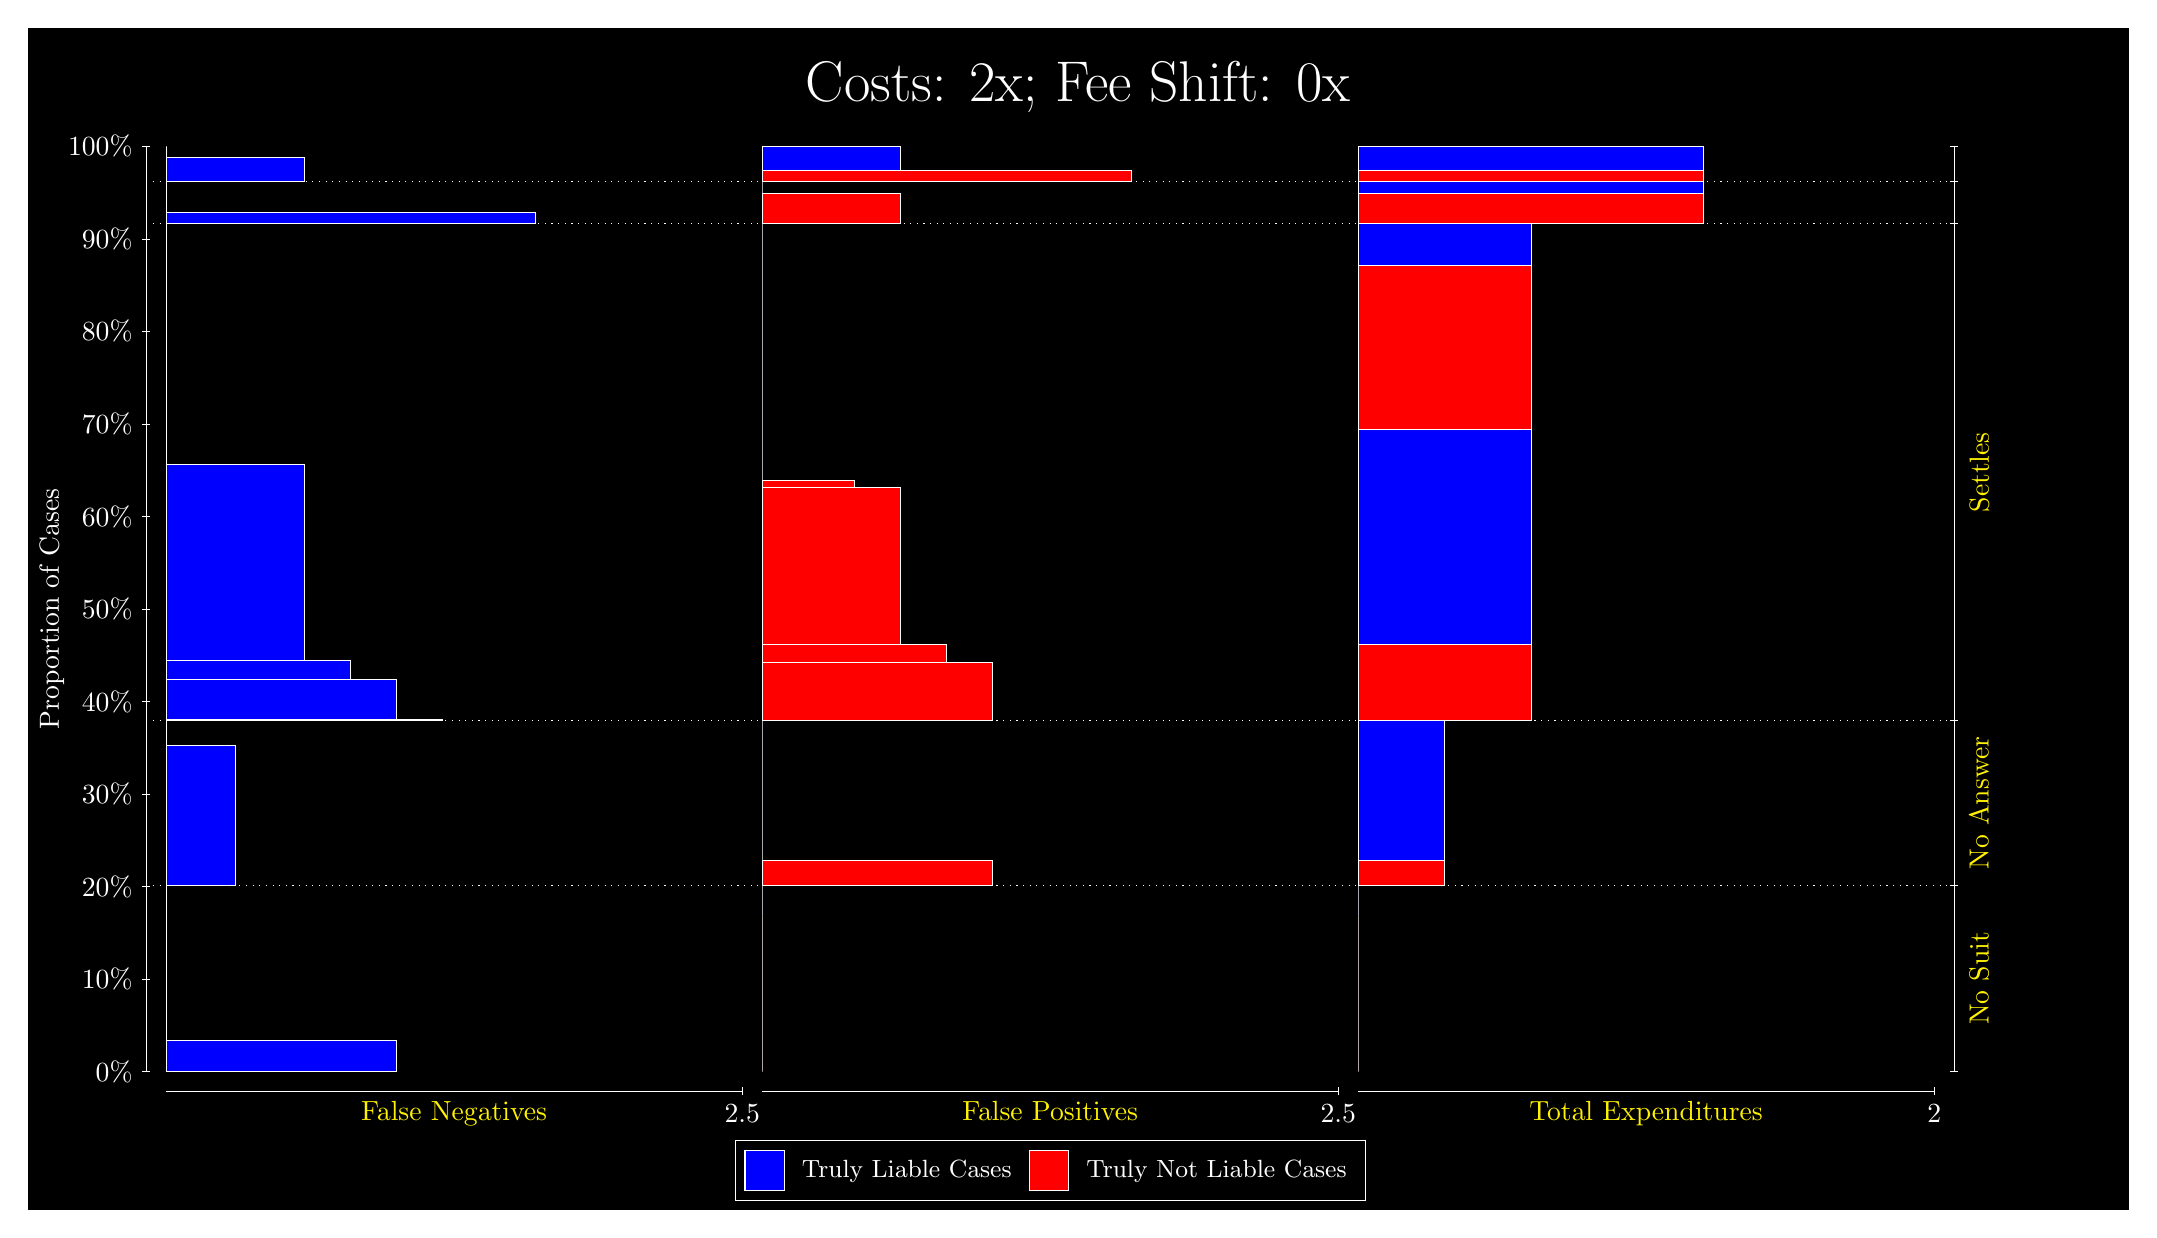
\begin{tikzpicture}
\draw[fill=black] (0,0) rectangle (26.667,15);
\draw[text=white] (0,13.5) rectangle (26.667,15) node[midway] {\huge Costs: 2x; Fee Shift: 0x};
\draw[white, very thin] (1.5,1.75) -- (1.5,13.5);
\node[rotate=90, text=white, anchor=center] at (0.3, 7.625) {Proportion of Cases};
\draw[white, very thin] (1.45,1.75) -- (1.55,1.75);
\node[text=white, anchor=east] at (1.45, 1.75) {0\%};
\draw[white, very thin] (1.45,2.925) -- (1.55,2.925);
\node[text=white, anchor=east] at (1.45, 2.925) {10\%};
\draw[white, very thin] (1.45,4.1) -- (1.55,4.1);
\node[text=white, anchor=east] at (1.45, 4.1) {20\%};
\draw[white, very thin] (1.45,5.275) -- (1.55,5.275);
\node[text=white, anchor=east] at (1.45, 5.275) {30\%};
\draw[white, very thin] (1.45,6.45) -- (1.55,6.45);
\node[text=white, anchor=east] at (1.45, 6.45) {40\%};
\draw[white, very thin] (1.45,7.625) -- (1.55,7.625);
\node[text=white, anchor=east] at (1.45, 7.625) {50\%};
\draw[white, very thin] (1.45,8.8) -- (1.55,8.8);
\node[text=white, anchor=east] at (1.45, 8.8) {60\%};
\draw[white, very thin] (1.45,9.975) -- (1.55,9.975);
\node[text=white, anchor=east] at (1.45, 9.975) {70\%};
\draw[white, very thin] (1.45,11.15) -- (1.55,11.15);
\node[text=white, anchor=east] at (1.45, 11.15) {80\%};
\draw[white, very thin] (1.45,12.325) -- (1.55,12.325);
\node[text=white, anchor=east] at (1.45, 12.325) {90\%};
\draw[white, very thin] (1.45,13.5) -- (1.55,13.5);
\node[text=white, anchor=east] at (1.45, 13.5) {100\%};

\draw[white, very thin] (24.457,1.75) -- (24.457,13.5);
\draw[white, very thin] (24.407,1.75) -- (24.507,1.75);
\node[anchor=west] at (24.407, 1.75) {};
\draw[white, very thin] (24.407,4.1137) -- (24.507,4.1137);
\node[anchor=west] at (24.407, 4.1137) {};
\draw[white, very thin] (24.407,6.2063) -- (24.507,6.2063);
\node[anchor=west] at (24.407, 6.2063) {};
\draw[white, very thin] (24.407,12.517) -- (24.507,12.517);
\node[anchor=west] at (24.407, 12.517) {};
\draw[white, very thin] (24.407,13.052) -- (24.507,13.052);
\node[anchor=west] at (24.407, 13.052) {};
\draw[white, very thin] (24.407,13.5) -- (24.507,13.5);
\node[anchor=west] at (24.407, 13.5) {};

\draw[white, very thin, fill=blue] (1.75,1.75) rectangle (4.6775,2.1429);
\draw[white, very thin, fill=red] (1.75,2.1429) rectangle (1.75,4.1137);
\draw[white, very thin, fill=blue] (1.75,4.1137) rectangle (2.6283,5.8892);
\draw[white, very thin, fill=red] (1.75,5.8892) rectangle (1.75,6.2063);
\draw[white, very thin, fill=blue] (1.75,6.2063) rectangle (5.2631,6.2197);
\draw[white, very thin, fill=blue] (1.75,6.2197) rectangle (4.6775,6.7285);
\draw[white, very thin, fill=blue] (1.75,6.7285) rectangle (4.092,6.9687);
\draw[white, very thin, fill=blue] (1.75,6.9687) rectangle (3.5065,9.4644);
\draw[white, very thin, fill=red] (1.75,9.4644) rectangle (1.75,12.517);
\draw[white, very thin, fill=blue] (1.75,12.517) rectangle (6.4341,12.663);
\draw[white, very thin, fill=red] (1.75,12.663) rectangle (1.75,13.052);
\draw[white, very thin, fill=blue] (1.75,13.052) rectangle (3.5065,13.355);
\draw[white, very thin, fill=red] (1.75,13.355) rectangle (1.75,13.5);
\draw[white, very thin, fill=red] (9.3189,1.75) rectangle (9.3189,3.7207);
\draw[white, very thin, fill=blue] (9.3189,3.7207) rectangle (9.3189,4.1137);
\draw[white, very thin, fill=red] (9.3189,4.1137) rectangle (12.246,4.4307);
\draw[white, very thin, fill=blue] (9.3189,4.4307) rectangle (9.3189,6.2063);
\draw[white, very thin, fill=red] (9.3189,6.2063) rectangle (12.246,6.9471);
\draw[white, very thin, fill=red] (9.3189,6.9471) rectangle (11.661,7.1761);
\draw[white, very thin, fill=red] (9.3189,7.1761) rectangle (11.075,9.1639);
\draw[white, very thin, fill=red] (9.3189,9.1639) rectangle (10.49,9.259);
\draw[white, very thin, fill=blue] (9.3189,9.259) rectangle (9.3189,12.517);
\draw[white, very thin, fill=red] (9.3189,12.517) rectangle (11.075,12.907);
\draw[white, very thin, fill=blue] (9.3189,12.907) rectangle (9.3189,13.052);
\draw[white, very thin, fill=red] (9.3189,13.052) rectangle (14.003,13.197);
\draw[white, very thin, fill=blue] (9.3189,13.197) rectangle (11.075,13.5);
\draw[white, very thin, fill=red] (16.888,1.75) rectangle (16.888,3.7207);
\draw[white, very thin, fill=blue] (16.888,3.7207) rectangle (16.888,4.1137);
\draw[white, very thin, fill=red] (16.888,4.1137) rectangle (17.986,4.4307);
\draw[white, very thin, fill=blue] (16.888,4.4307) rectangle (17.986,6.2063);
\draw[white, very thin, fill=red] (16.888,6.2063) rectangle (19.083,7.1761);
\draw[white, very thin, fill=blue] (16.888,7.1761) rectangle (19.083,9.912);
\draw[white, very thin, fill=red] (16.888,9.912) rectangle (19.083,11.995);
\draw[white, very thin, fill=blue] (16.888,11.995) rectangle (19.083,12.517);
\draw[white, very thin, fill=red] (16.888,12.517) rectangle (21.279,12.907);
\draw[white, very thin, fill=blue] (16.888,12.907) rectangle (21.279,13.052);
\draw[white, very thin, fill=red] (16.888,13.052) rectangle (21.279,13.197);
\draw[white, very thin, fill=blue] (16.888,13.197) rectangle (21.279,13.5);
\draw[white, dotted] (1.5,4.1137) -- (24.457,4.1137);
\draw[white, dotted] (1.5,6.2063) -- (24.457,6.2063);
\draw[white, dotted] (1.5,12.517) -- (24.457,12.517);
\draw[white, dotted] (1.5,13.052) -- (24.457,13.052);
\draw[white, very thin] (1.75,1.5) -- (9.0689,1.5);
\node[text=yellow, anchor=north] at (5.4094, 1.5) {False Negatives};
\draw[white, very thin] (9.0689,1.45) -- (9.0689,1.55);
\node[text=white, anchor=north] at (9.0689, 1.45) {2.5};

\draw[white, very thin] (9.3189,1.5) -- (16.638,1.5);
\node[text=yellow, anchor=north] at (12.978, 1.5) {False Positives};
\draw[white, very thin] (16.638,1.45) -- (16.638,1.55);
\node[text=white, anchor=north] at (16.638, 1.45) {2.5};

\draw[white, very thin] (16.888,1.5) -- (24.207,1.5);
\node[text=yellow, anchor=north] at (20.547, 1.5) {Total Expenditures};
\draw[white, very thin] (24.207,1.45) -- (24.207,1.55);
\node[text=white, anchor=north] at (24.207, 1.45) {2};

\node[text=yellow, centered, rotate=90] at (24.777, 2.9318) {No Suit};
\node[text=yellow, centered, rotate=90] at (24.777, 5.16) {No Answer};
\node[text=yellow, centered, rotate=90] at (24.777, 9.3617) {Settles};



\draw (12.978300999999998,1.5) node[draw=none] (baseCoordinate) {};
\begin{scope}[align=center]
        \matrix[scale=0.5, draw=white, below=0.5cm of baseCoordinate, nodes={draw}, column sep=0.1cm]{
            \node[rectangle, draw, minimum width=0.5cm, minimum height=0.5cm, fill=blue] {}; &
            \node[draw=none, font=\small, text=white] (B) {Truly Liable Cases}; &
            \node[rectangle, draw, minimum width=0.5cm, minimum height=0.5cm, fill=red] {}; &
            \node[draw=none, font=\small, text=white] (B) {Truly Not Liable Cases}; \\
            };
\end{scope}

\end{tikzpicture}
\end{document}